\documentclass[11pt]{article}
\usepackage[a4paper,margin=2.5cm]{geometry}
\usepackage[T1]{fontenc}
\usepackage[utf8]{inputenc}
\usepackage{amsmath,amssymb}
\usepackage{booktabs,array}
\usepackage{graphicx}
\usepackage{xcolor}
\usepackage{listings}
\usepackage[numbers,sort&compress]{natbib}
\usepackage[colorlinks=true,linkcolor=blue!50!black,citecolor=blue!50!black,urlcolor=blue!50!black]{hyperref}
\lstset{basicstyle=\ttfamily\small,columns=fullflexible,frame=single,framerule=0.3pt,
  rulecolor=\color{black!30},xleftmargin=4pt,xrightmargin=4pt}

\newcommand{\qZ}{qg_Z}

\title{Training quantum neural networks for T1-limited hardware:\\
what the qg symmetry filter does and does not do}
\author{Vicente Humberto Monteverde\\
\small Universidad del Museo Social Argentino (UMSA), Argentina\\
\small ORCID 0000-0001-8884-4811}
\date{\small Draft of 2 October 2026}

\begin{document}
\sloppy
\maketitle

\begin{abstract}
A quantum neural network (QNN) built from gates that conserve the Hamming weight keeps its data in one
weight sector, so the shots that left the sector can be discarded at readout. This is the qg filter of
the qang library~\cite{monteverde2026qang,monteverde2026witness}. We show that, with equal amplitude damping
(T1) on every qubit, the filtered readout of such a network is exactly the noiseless one in any weight
sector. The kept fraction of shots is $(1-\gamma)^{k\,d}$ for weight $k$ and depth $d$, and training under
T1 with the filter gives exactly the parameters of noiseless training. We then measure what this is worth
on four small classification datasets. Every result is reported with the filter and without it, and every
prediction was committed before its run, failures included. Over 60 runs per model, a network trained on a
simulator and run under T1 gains $+2.5$ points from the filter at weight~1 (95\% CI $[0.8,4.1]$) and
$+16.5$ points at weight~2 ($[11.8,21.2]$), recovering its noiseless accuracy exactly. A network trained
under the calibrated noise without the filter catches up (differences of $0.1$ points), and the filter
corrects neither dephasing nor unequal T1 across qubits. These models are classically simulable and no
quantum advantage is claimed. The filter is a way to make noise-free training valid under relaxation, at a
shot cost known in advance. The models are released as \texttt{qang.qml} (version 0.6.0,
\texttt{pip install qang}).
\end{abstract}

\section{Introduction}

Variational quantum classifiers are trained on simulators and run on noisy devices, or trained directly
under device noise. Noise-aware training~\cite{wang2022quantumnat} is the usual remedy when the two
differ. Symmetry verification~\cite{bonetmonroig2018,mcardle2019} is a different remedy: when the ideal
circuit conserves a quantity, outcomes that violate it can be discarded. The qang project expresses
qubit readouts in qg units ($\qZ=\langle\sigma_z\rangle$ and its companions)~\cite{monteverde2026qang}. It
built a register-mean witness and a shot-level filter for circuits that conserve a Hamming
weight~\cite{monteverde2026witness}. This note asks a narrow question: for a QNN that conserves the weight,
how much does that filter change the accuracy of a classifier on T1-limited hardware, and when does it stop
mattering?

We answer with exact simulation, a fixed protocol and an explicit comparison. Every reading is taken with
qang (filtered) and without it (raw), on the same trained parameters or the same initialization. The
predictions of every study were committed to the repository before the run that tested them. Of 27
pre-registered predictions in the studies summarized here, 22 passed and 5 failed; the failures are
reported alongside the passes.

\section{Model and theory}

\paragraph{Weight-conserving QNN.} On $n$ qubits, a reconfigurable beam splitter (RBS) gate acts on a pair
$(a,b)$ as a Givens rotation between $|10\rangle$ and $|01\rangle$ and leaves $|00\rangle$ and $|11\rangle$
fixed, so it conserves the Hamming weight~\cite{landman2022}. We use $n=5$ and three layers of RBS gates on
the pairs $\{(0,1),(2,3)\}$, $\{(1,2),(3,4)\}$, $\{(4,0)\}$. That gives 15 angles and depth $d=9$ (sublayers).
The readout is $z=\sum_i c_i\,\qZ^{(i)}+b$ with trainable $c_i,b$ and a logistic loss.

\paragraph{Encodings.} With four features $x\in[-1,1]^4$ let $v=(x,1)/\|(x,1)\|$; the constant component
keeps $\|x\|$. Model E (weight~1) puts $v_i$ on the basis state with qubit $i$ excited. Model W (weight~2)
puts $v_iv_j$ on the state with qubits $i<j$ excited, normalized. The sectors have dimensions 5 and 10.

\paragraph{The filter.} With qang, the readout keeps only the shots whose weight equals the input weight $k$
and renormalizes (\texttt{qang.sectors.filter\_distribution}). Without qang, all shots are used.

\paragraph{F1/F4: exactness under equal T1.} Let amplitude damping with probability $\gamma$ act on every
qubit after every sublayer. Its no-jump Kraus operator multiplies a basis state with $k$ excitations by
$(1-\gamma)^{k/2}$: the same factor for every state in the weight-$k$ sector. Every jump lowers the weight
and leaves the sector. The weight-conserving gates never bring a lowered state back. So, conditioned on the
weight being $k$, the state is exactly the noiseless one, and
\begin{equation}
  \text{kept fraction}=(1-\gamma)^{k\,d}.
\end{equation}
For $\gamma=0.08$ and $d=9$ this is $0.472$ at weight~1 and $0.223$ at weight~2. If the damping differs
between qubits, the no-jump factor is $\prod_{q\in S}(1-\gamma_q)^{1/2}$ over the excited set $S$, which is
not uniform, and exactness is lost. Dephasing conserves the weight, so the filter cannot see it.

\paragraph{F3: training.} Since the filtered T1 readout equals the noiseless one for every parameter value,
the loss and all gradients are identical. Training under T1 with the filter therefore yields the parameters
of noiseless training from the same initialization.

\paragraph{F2: simulability.} At weight~1 the network is a $5\times5$ orthogonal matrix $O$ on $v$, and $z$ is
a quadratic form in $v$. At weight $k$ the sector has dimension $\binom{n}{k}$, polynomial for fixed $k$.
These models can be simulated classically. Whether larger, higher-weight versions could not be is a separate
question~\cite{cerezo2023simulability} that this note does not address.

\section{Methods}

Datasets (binary): iris (versicolor vs virginica), breast cancer, wine (classes 0 vs 1) and digits (3 vs 8),
with 100 samples per class where available. Each run uses a stratified 70/30 split, standardization, PCA to
four components where needed, and scaling to $[-1,1]$; one test sample is worth 2--3 points. Training uses
Adam for 120 epochs, with central-difference gradients on the angles. Noise conditions are applied after every
sublayer: equal T1 with $\gamma=0.08$; unequal T1 with $\gamma_q$ from 0.04 to 0.12 (mean 0.08); and equal
T1 plus a phase flip with probability 0.03. The simulation is exact. T1 and dephasing keep the density matrix
block-diagonal in the Hamming weight, so one block per weight is propagated; this is checked against the full
density matrix to $10^{-12}$. Protocol: each study's script, with its predictions written in the header, was
committed before the seed of its reported run was used; code was debugged on another seed with few epochs.
The commit hashes are in the research notes~\cite{monteverde2026qang}.

\section{Results}

\paragraph{Single-seed studies.} The weight-conserving QNN that keeps the norm reaches a mean accuracy of
0.960 over the four datasets. That is level with a standard (non-conserving) four-qubit QNN (0.952) and with
an RBF support-vector machine (0.957) and a small MLP (0.961). Without the norm component the same network
gets 0.791. Trained noiselessly and run under T1 with the filter, it keeps exactly its noiseless accuracy.
Training under T1 with the filter reproduces noiseless training to $5\times10^{-9}$ in the parameters (F3).
At $\gamma=0.08$, a standard QNN trained noiselessly collapses under T1 (0.771); trained under T1 it
recovers (0.944).

The predictions that failed:
\begin{itemize}
\item arccos encoding gave no accuracy gain;
\item the classical quadratic twin did not match the QNN within 1 point at default regularization;
\item unequal T1 cost the filter 1.5 points in one run (bound: 1 point);
\item weight~2 was less accurate than weight~1 (by 3.7 points);
\item trained under T1, the weight-2 model without the filter was 0.6 points ahead of the filtered one.
\end{itemize}

\paragraph{Replication over 60 runs.} The key comparisons were repeated over 5 seeds $\times$ 3 splits
$\times$ 4 datasets. Table~\ref{tab:main} and Fig.~\ref{fig:main} give the results; all five
pre-registered predictions of this replication passed.

\begin{table}[h]
\centering\small
\begin{tabular}{lcccc}
\toprule
 & \multicolumn{2}{c}{E (weight 1)} & \multicolumn{2}{c}{W (weight 2)}\\
reading & with qang & without & with qang & without\\
\midrule
exact (no noise) & 0.952 & & 0.922 & \\
T1, trained without noise & 0.952 & 0.928 & 0.922 & 0.757\\
T1, trained under the noise & 0.952 & 0.951 & 0.922 & 0.924\\
unequal T1, trained without noise & 0.947 & 0.921 & 0.916 & 0.732\\
dephasing, trained without noise & 0.918 & 0.792 & 0.882 & 0.656\\
dephasing, trained under the noise & 0.950 & & 0.926 & \\
\bottomrule
\end{tabular}
\caption{Mean test accuracy over 60 runs per model, with and without the qg filter.}
\label{tab:main}
\end{table}

\begin{figure}[h]
\centering
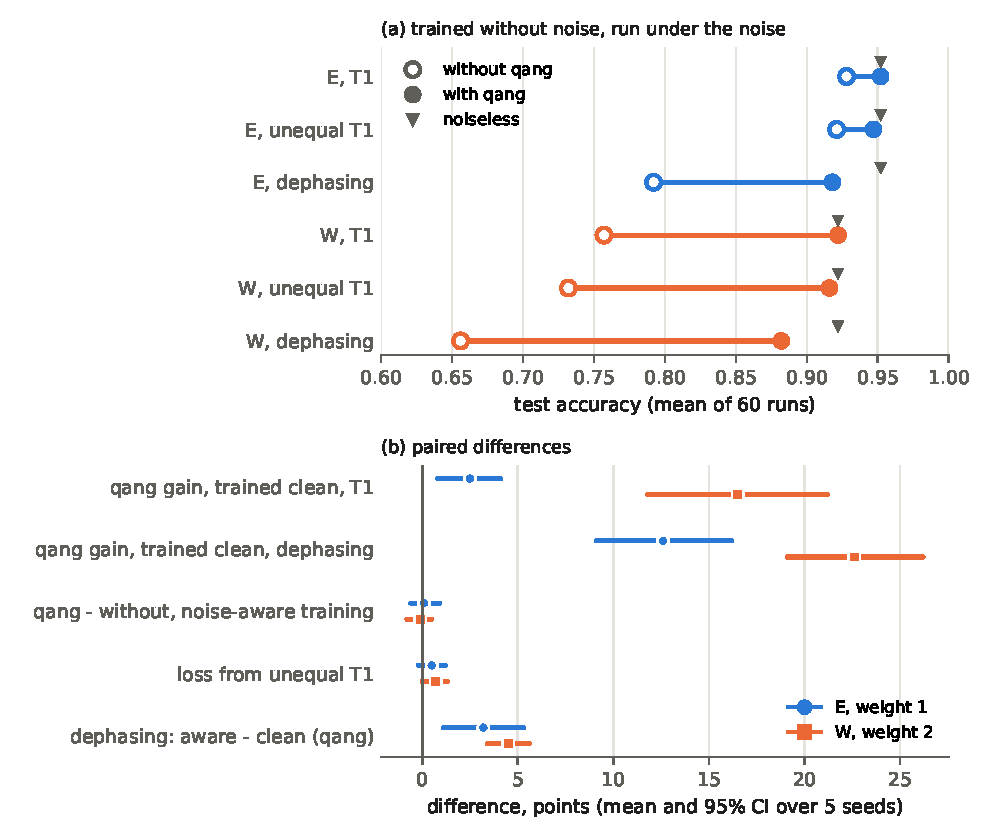
\includegraphics[width=0.86\textwidth]{fig_qml.pdf}
\caption{(a) Accuracy of networks trained without noise and run under the noise, without (open) and with
(filled) the filter; triangles mark the noiseless accuracy. (b) Paired differences, mean and 95\% CI across
5 seeds.}
\label{fig:main}
\end{figure}

The paired differences (mean, 95\% CI across seeds) were as follows.
\begin{itemize}
\item \textit{Gain from the filter, trained without noise, under T1:} $+2.5$ $[0.8,4.1]$ points (E) and
  $+16.5$ $[11.8,21.2]$ (W). The filtered model was ahead or tied in 50/60 (E) and 56/60 (W) runs.
\item \textit{With noise-aware training:} $+0.1$ $[-0.6,0.9]$ (E) and $-0.1$ $[-0.8,0.5]$ (W).
\item \textit{Loss from unequal T1:} $0.5$ $[-0.2,1.2]$ (E) and $0.7$ $[0.0,1.3]$ (W). The 1.5 points of the
  earlier run were at the top of the spread.
\item \textit{Dephasing, noise-aware minus clean training with the filter:} $+3.2$ (E) and $+4.5$ (W),
  both CIs above 0.
\item \textit{Under dephasing, a model trained without noise still gains} $+12.6$ (E) and $+22.6$ (W) points
  from the filter, which removes the T1 part of the combined noise.
\item \textit{Weight~2 against weight~1:} $-3.0$ $[-4.0,-2.0]$ points.
\end{itemize}

\section{Discussion}

The difference the filter makes depends on how the network was trained. Trained on a simulator and run
under relaxation, the filter is decisive. Its effect grows with the weight, because a weight-$k$ state decays
$k$ times faster. Trained under a calibrated noise model, a network without the filter learns the decay, and
the filter adds nothing measurable. What the filter provides is therefore procedural rather than an accuracy
gain over the best alternative. Under equal T1 it makes noise-free training exactly valid, with no noise
model and no noisy training runs, and its cost (the discarded shots) is known before running. Unequal T1 and
dephasing are not corrected. On hardware with a large spread of T1 or strong dephasing, the filter
complements a noise model and does not replace it.

\paragraph{Limitations.} All noise is simulated. There is one architecture per weight, five qubits, and
small datasets in which one test sample is worth 2--3 points. The weight-2 encoding is one choice among many,
and it did not use the larger sector well. No quantum advantage is claimed: these networks are classically
simulable. A hardware run with the filter is the natural next test.

\section*{Code and data availability}

Models: \texttt{qang.qml} in \texttt{qang} 0.6.0 (\texttt{pip install qang}), NumPy only, with
\texttt{WeightQNN}, \texttt{kept\_fraction} and \texttt{compare\_qang}. Studies:
\texttt{examples/qnn\_*\_qg.py} and RESEARCH\_NOTES \S75--\S80, with tests in \texttt{tests/}. The Colab
notebooks \texttt{notebooks/qang\_qml.ipynb} (English) and \texttt{qang\_qml\_es.ipynb} (Spanish) install the
library from PyPI. Repository: \url{https://github.com/Viny2030/qang}.

\begin{lstlisting}[language=Python]
from qang.qml import WeightQNN
m = WeightQNN(n_qubits=5, weight=2).fit(X_train, y_train)
m.score(X_test, y_test, gamma=0.08, qang=True)   # = noiseless accuracy
m.score(X_test, y_test, gamma=0.08, qang=False)  # raw readout
\end{lstlisting}

\bibliographystyle{unsrtnat}
\bibliography{../refs}

\end{document}
